\newcommand{\teaserFig}{
  \teaser{
		\centering
		\begin{subfigure}[t]{.3\textwidth}
			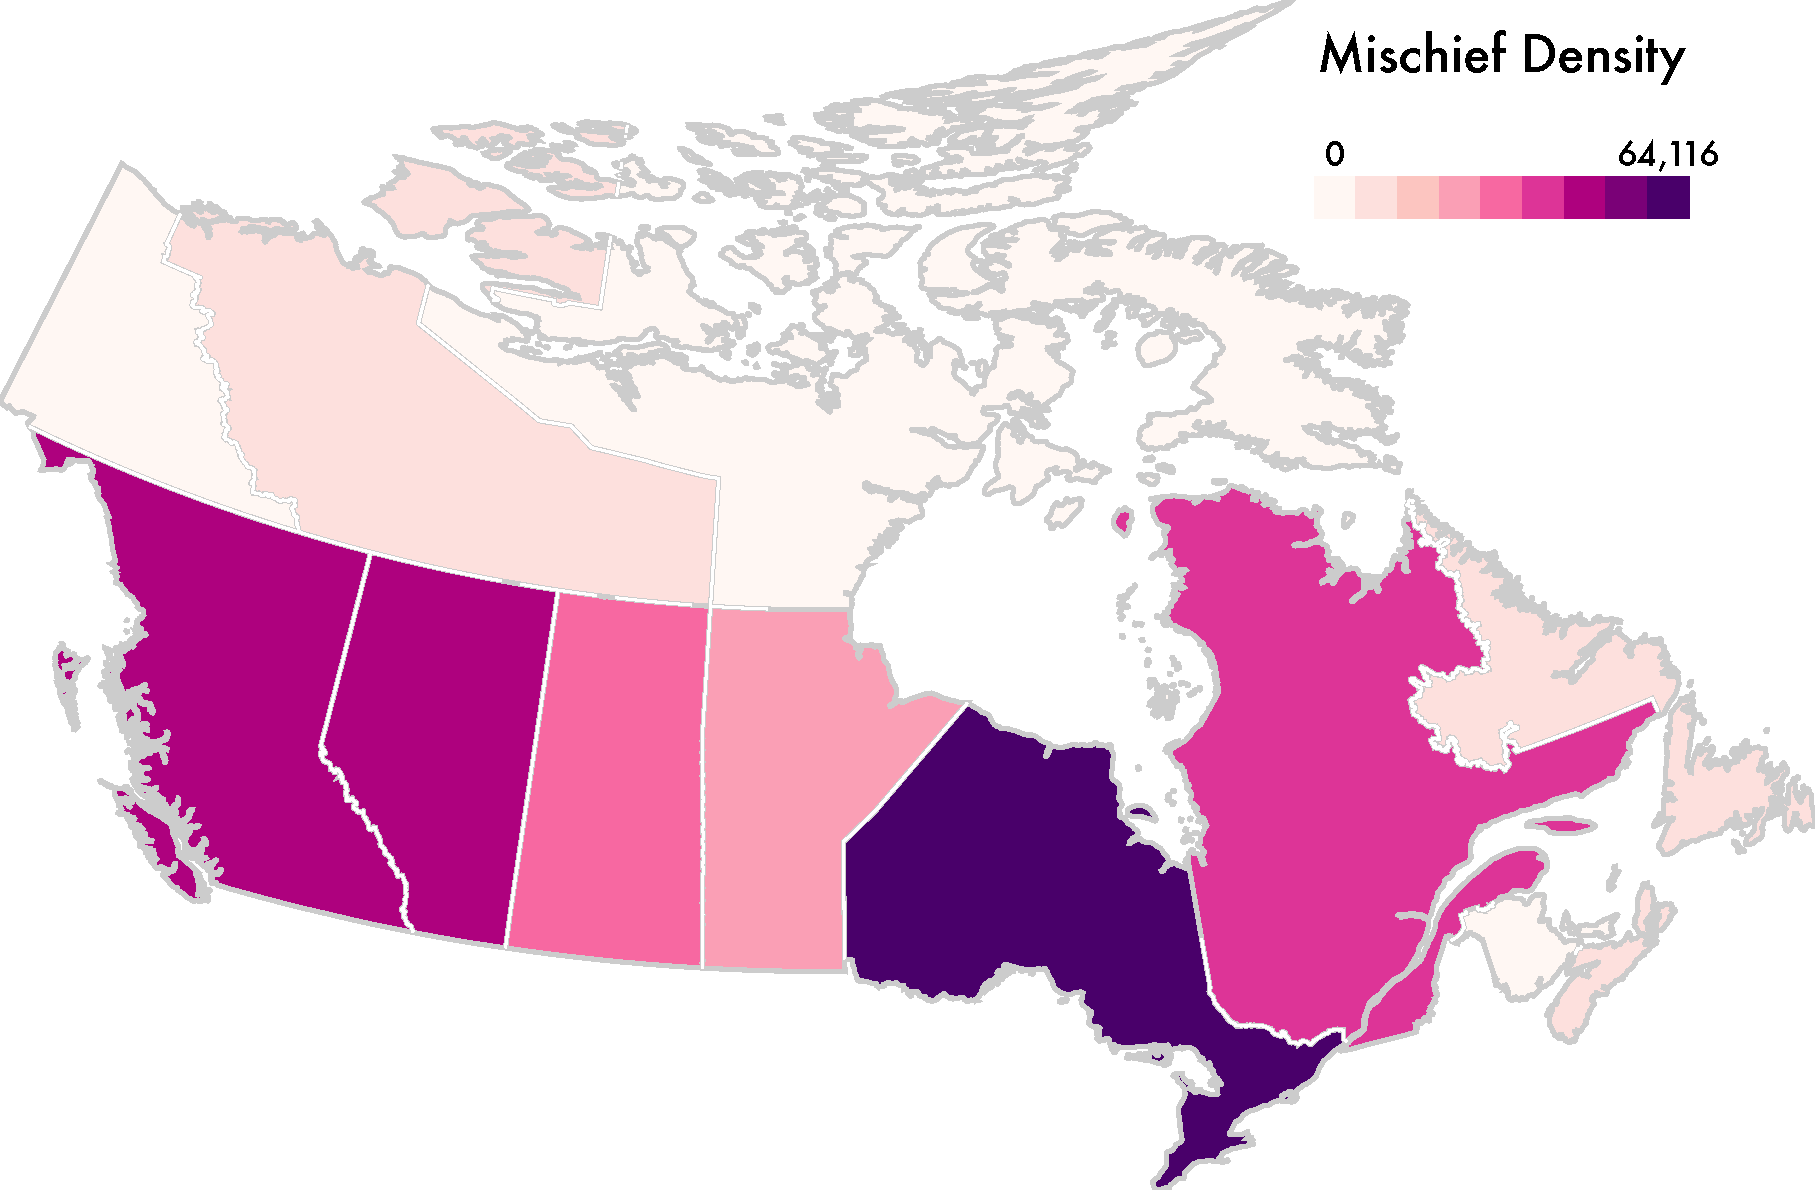
\includegraphics[width=\textwidth]{figures/canada-density}
			\caption{The \textbf{Event Density} of ``mischief'' in Canada.}
			\label{fig:canadadensity}
		\end{subfigure}
		~
		\begin{subfigure}[t]{.3\textwidth}
			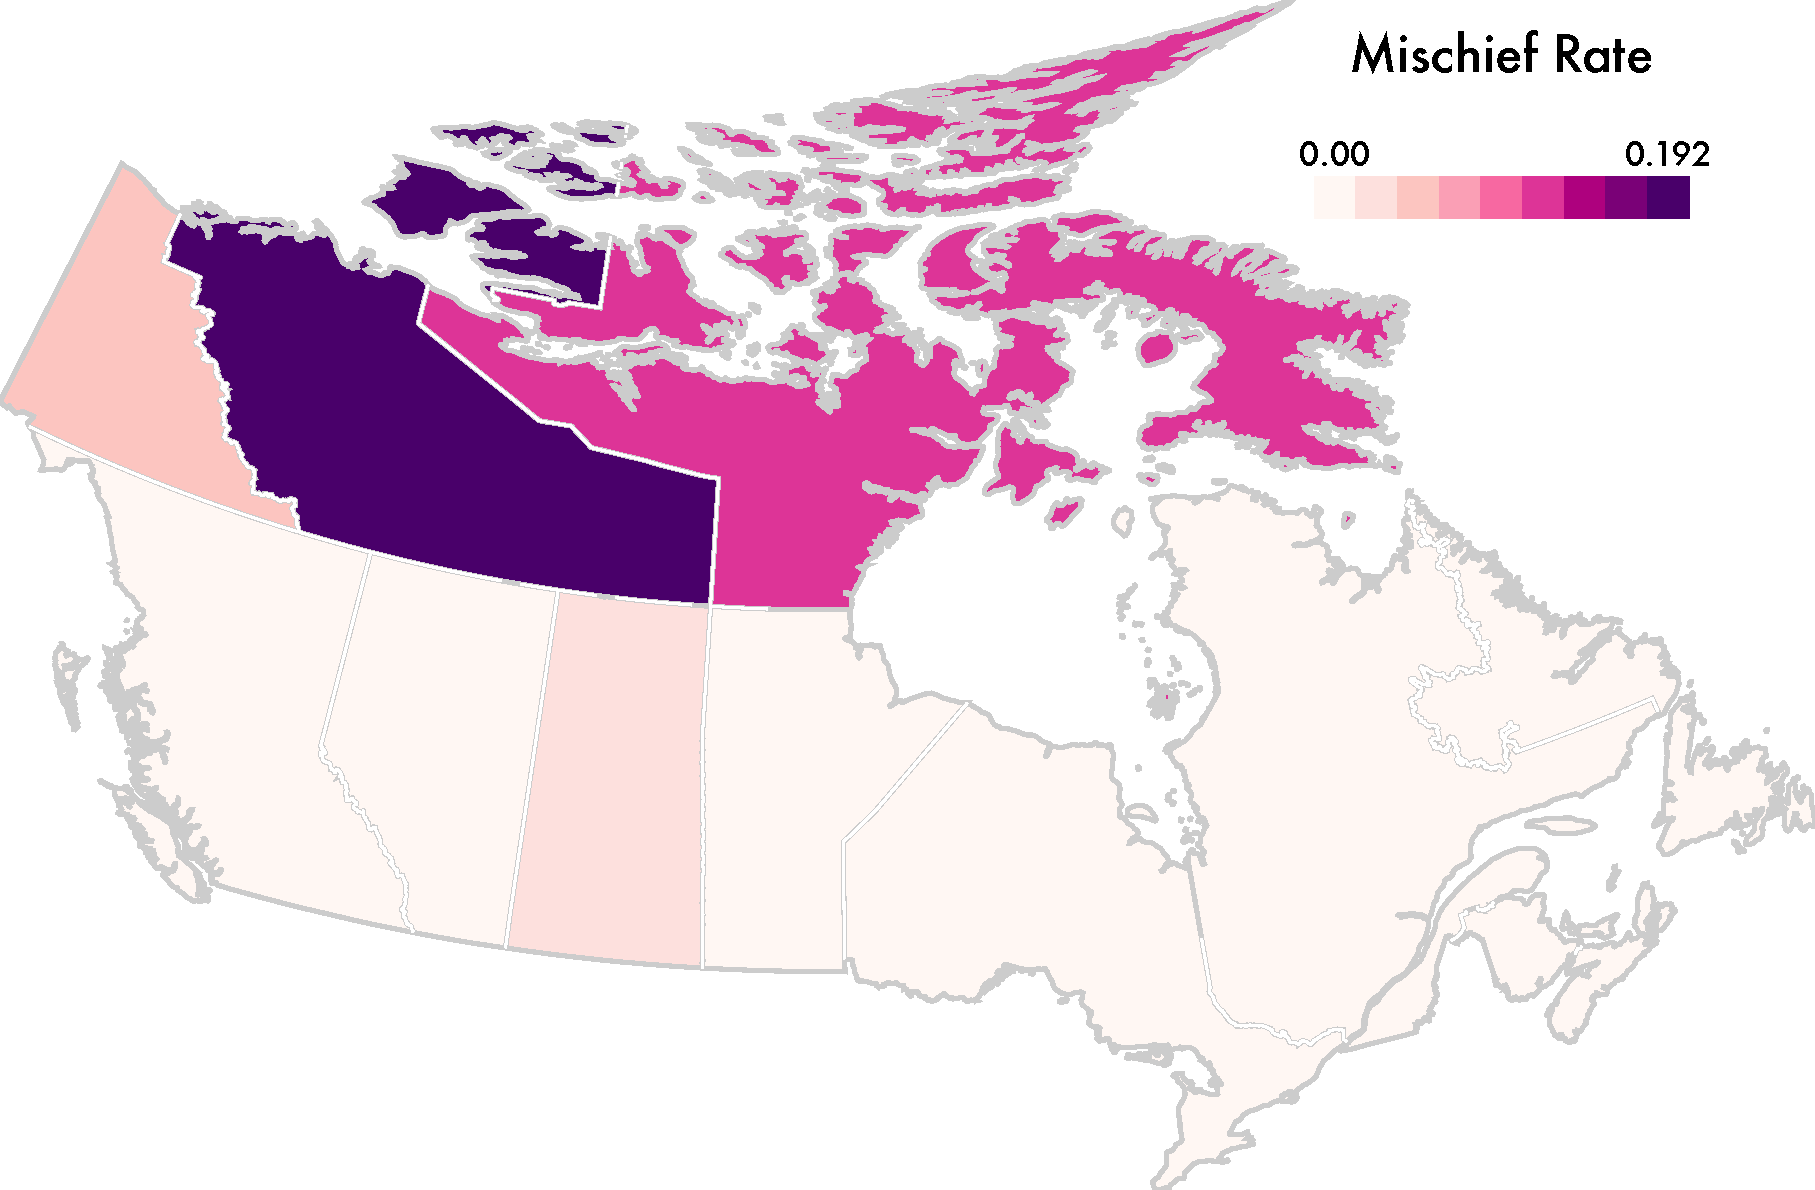
\includegraphics[width=\textwidth]{figures/canada-rate}
			\caption{The per-capita \textbf{Event Rate} of mischief.}
			\label{fig:canadarate}
		\end{subfigure}
		~
		\begin{subfigure}[t]{.3\textwidth}
			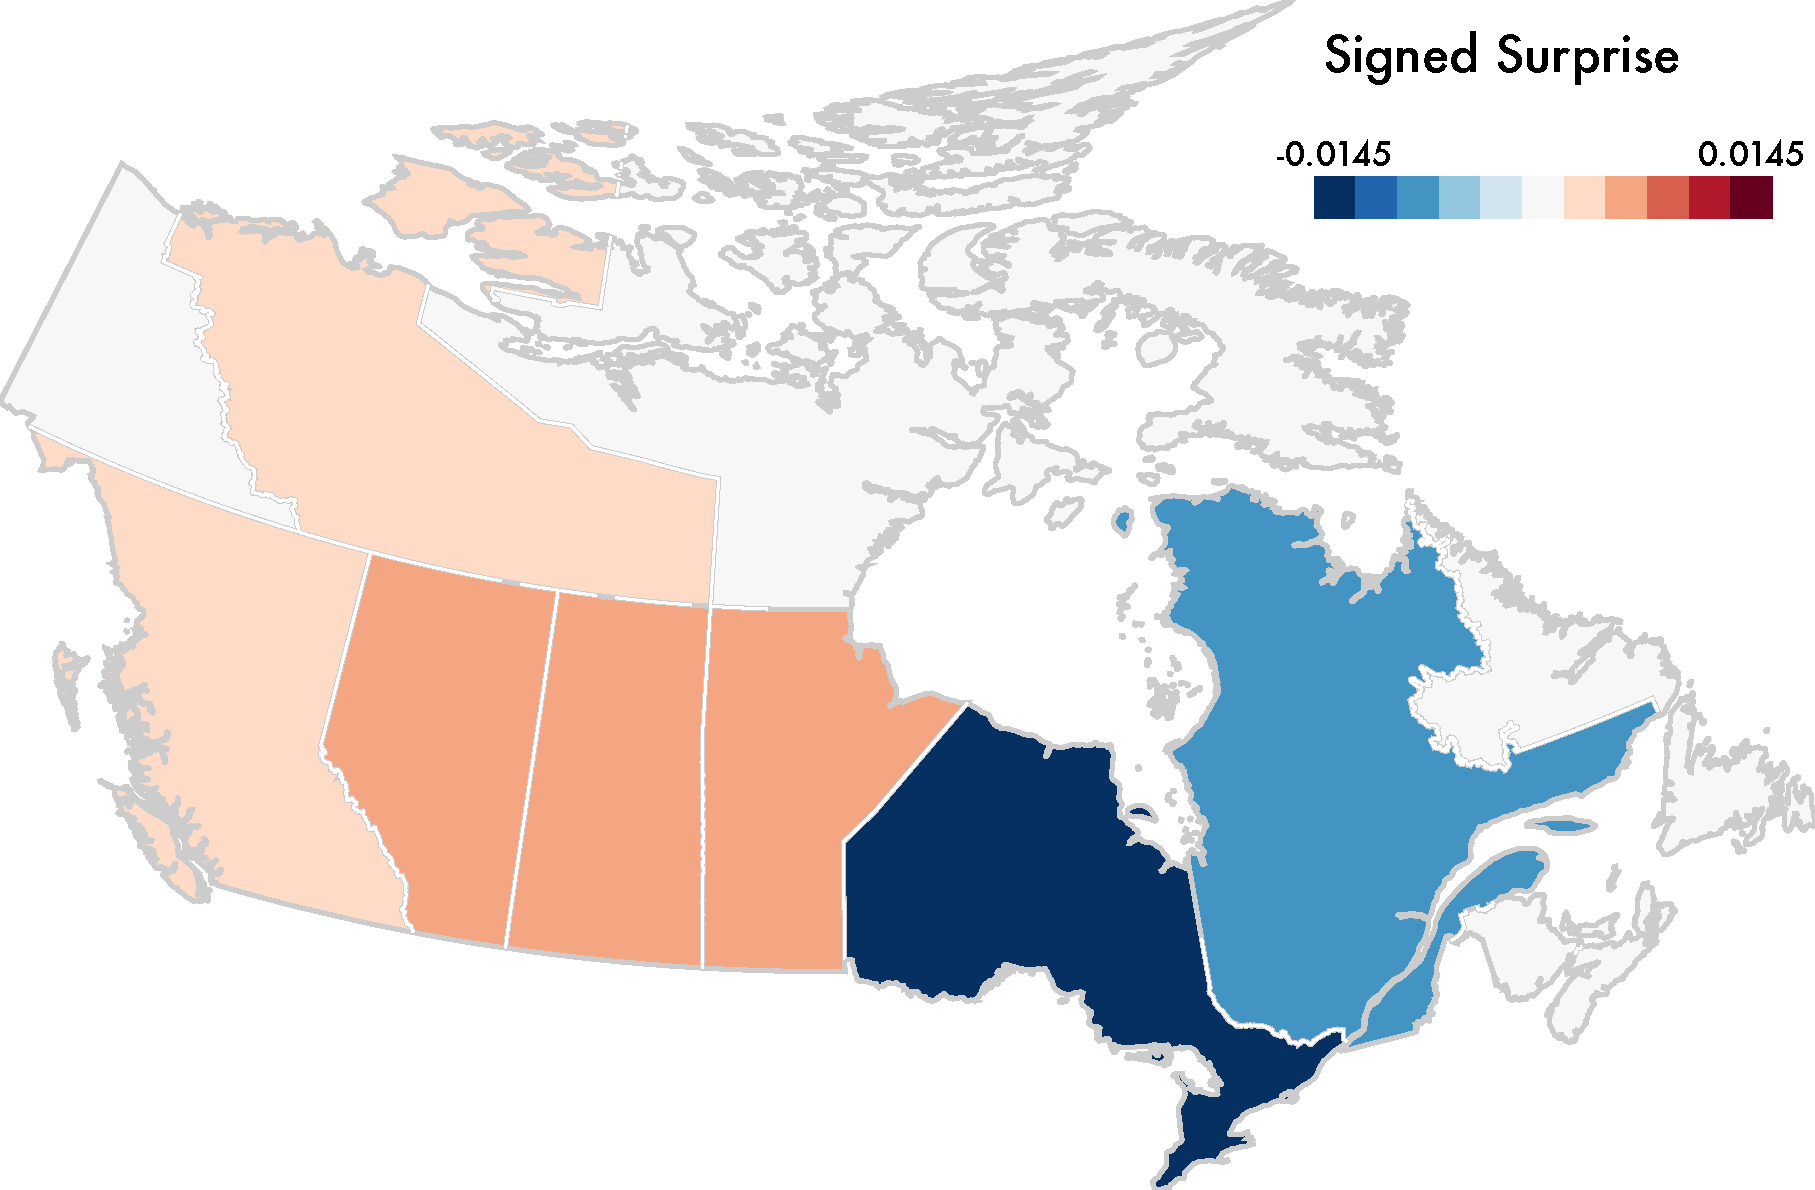
\includegraphics[width=\textwidth]{figures/canada-surprise2}
			\caption{The \textbf{Surprise Map} of mischief. }
			\label{fig:canadasurprise}
		\end{subfigure}
		\caption{ Choropleth maps of (a) event density, (b) per-capita event rates, and (c) Bayesian surprise for ``mischief'' (a class of property crime) in Canada. Which province or territory is safest? The density of crimes (Fig. \ref{fig:canadadensity}) in the southern provinces suggest that they are less safe; however, this is due to the much larger populations in those provinces. Normalizing to a per-capita rate (Fig. \ref{fig:canadarate}) gives the opposite impression. A Surprise Map (Fig. \ref{fig:canadasurprise}), using both population density and a de Moivre funnel as models, finds the provinces that stick out: Ontario and Quebec have crime rates lower than expected given their population. The seemingly high per-capita rates in Nunavut accord with the higher variability that can arise from a smaller population. }
	\label{fig:canada}
  }

}

\newcommand{\gaussFig}{
 \begin{figure*}
 \centering
 \includegraphics[width=.9\textwidth]{figures/gauss-2}
 \caption{
 	Changes in beliefs about spatial models leading to surprise. Here the events are sampled from a Gaussian distribution, and there are two proposed spatial models of events: a Gaussian (in this case, the correct model), and a uniform model. Initially, both models are equiprobable. However, as more events are processed, modes that are in keeping with a Gaussian model (but would be unlikely in a uniform model), adjust the modal beliefs in favor of the Gaussian model (causing surprise). Once the Gaussian model is established as the clear favorite, the surprise of events tapers off, asymptotically approaching 0. Probability histograms range from $[0,1]$, average surprise ranges from $[0,0.01]$ bits.
 }
 \label{fig:gauss}
 \end{figure*}
}

\newcommand{\funnelFig}{
	\begin{figure}
		\centering
		\includegraphics[width=.9\columnwidth]{figures/funnel}
		\caption{
			A funnel plot of the 2008 U.S. unemployment rate by county. The gray region depicts a 95\% confidence interval of the sample mean, using standard error. As sample size increases, variability decreases. Large differences in event rates may be an artifact of sample size. Conversely, small changes in event rate can be unexpected in high population regions. Some interesting counties (where $P(D|M)$ are low) are Imperial County, CA, which has a somewhat low population, but a high unemployment rate (30\%), and LA County, CA, which has an unemployment rate that is not much higher than the national average (12.7\%, versus an 8.7\% average), but is so populous that its higher rate is notable. Color encodes the unemployment rate, $[0,30\%]$.
		}
		\label{fig:funnel}
	\end{figure}
}


\newcommand{\gaussMaps}{
  \begin{figure}
  	\centering
    \includegraphics[width=.9\columnwidth]{figures/gauss2-2}
  	\caption{A Surprise Map from our synthetic dataset presented in \protect\S\ref{sec:synthetic}. The large heatmaps (top) show the signed surprise (left, from [-0.53,0.53]) and the KDE event density (right). The small heatmaps (bottom) show differences between observed data and the expectations provided by our spatial models. Blue regions are where we have seen fewer events than we expect, and red regions have more density than expected. After 250 events, belief in the Gaussian model is very close to 1. As such, the Surprise Map highlights deviations from the Gaussian model, in this case the red spatial outliers. Different model beliefs would produce a different weighting of events.
  	}
  	\label{fig:gaussMap}
  \end{figure}
}

\newcommand{\popFig}{
\begin{figure*}
	\centering
	\begin{subfigure}[tb]{0.3\textwidth}
		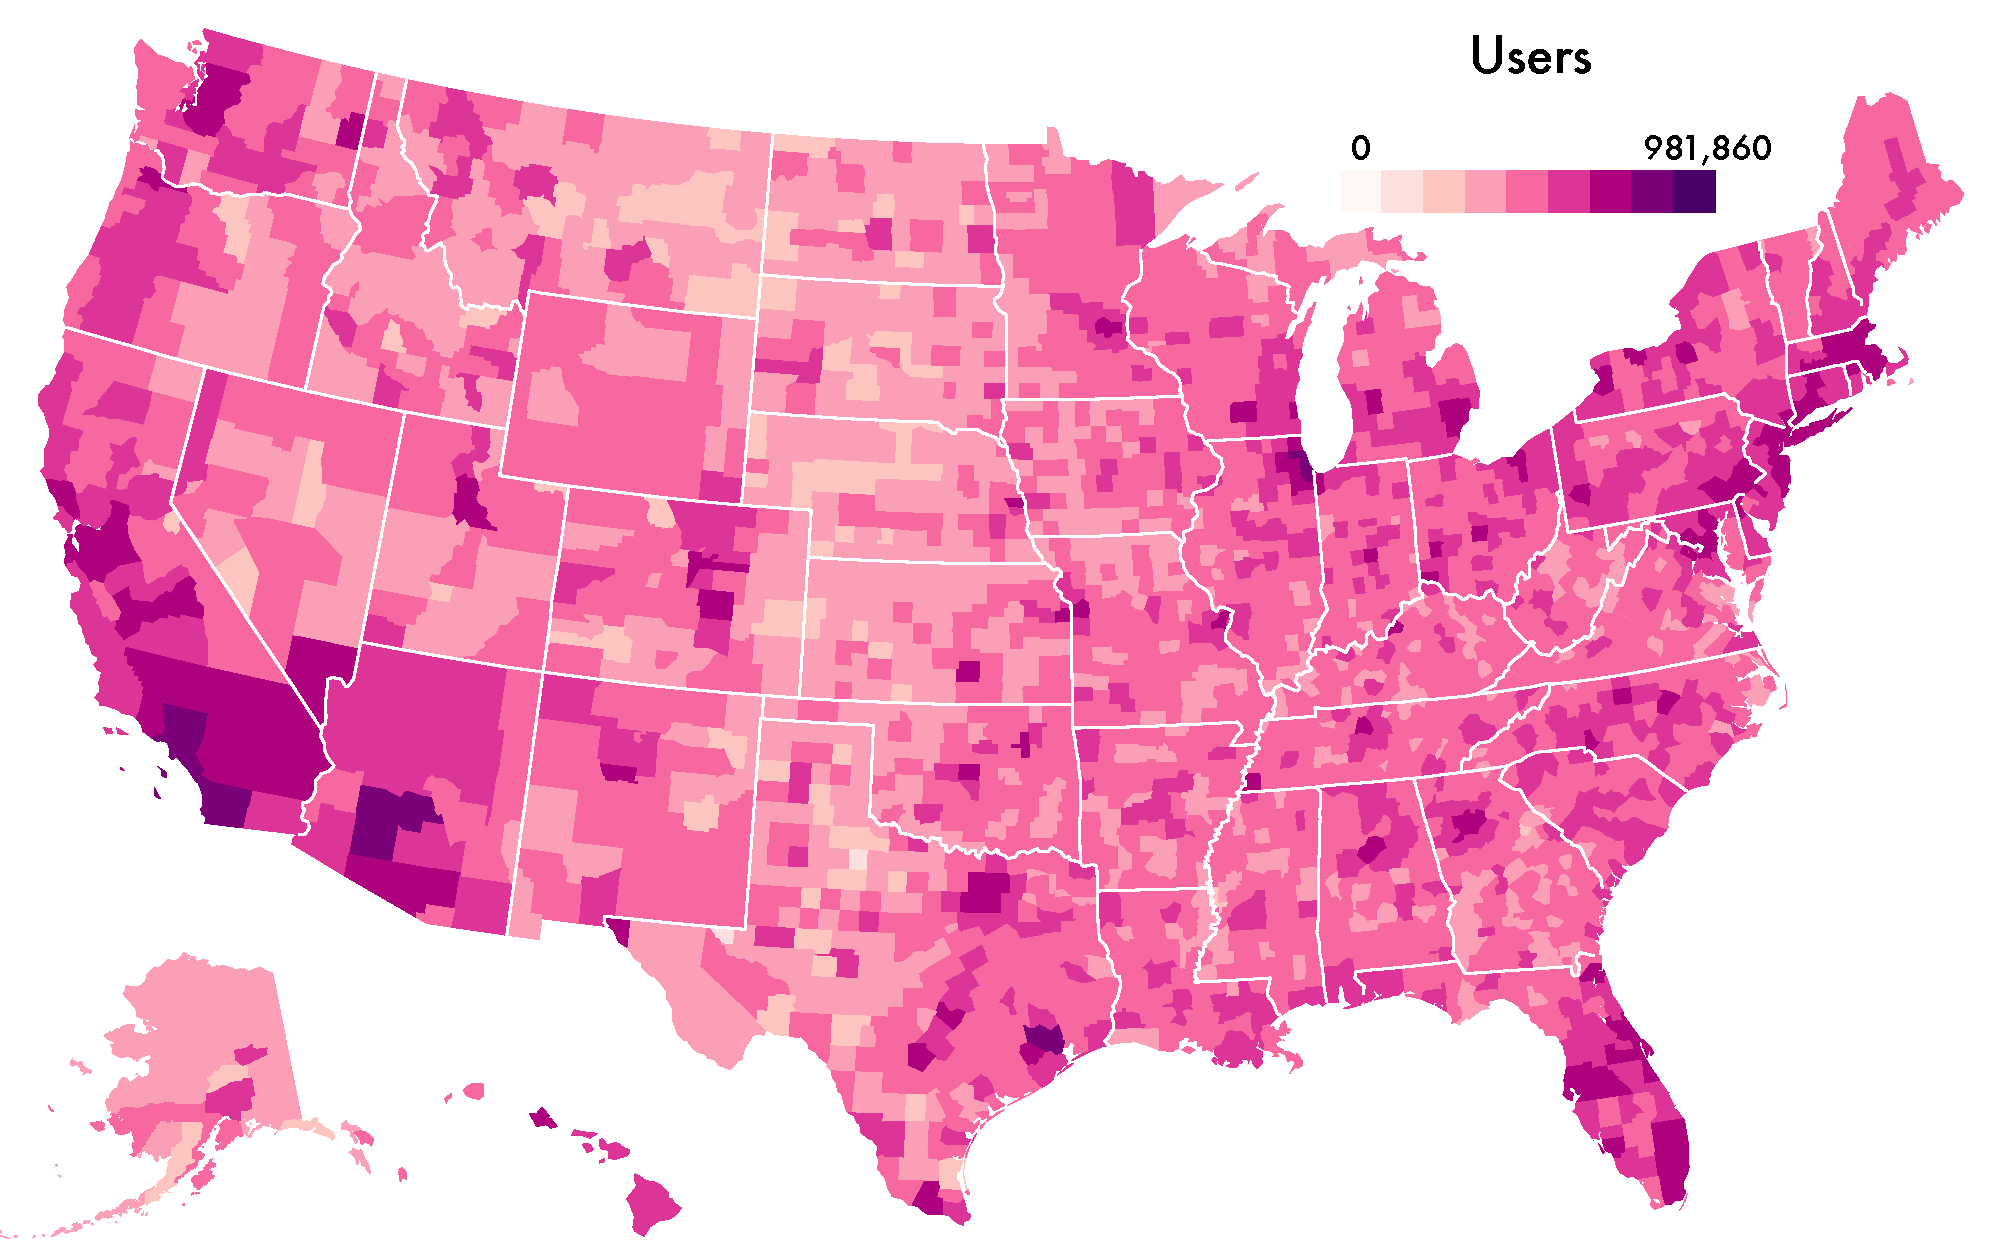
\includegraphics[width=\textwidth]{./figures/population1}
		\caption{Users of Application A}
		\label{fig:pop1}
	\end{subfigure}
	~
	\begin{subfigure}[tb]{0.3\textwidth}
		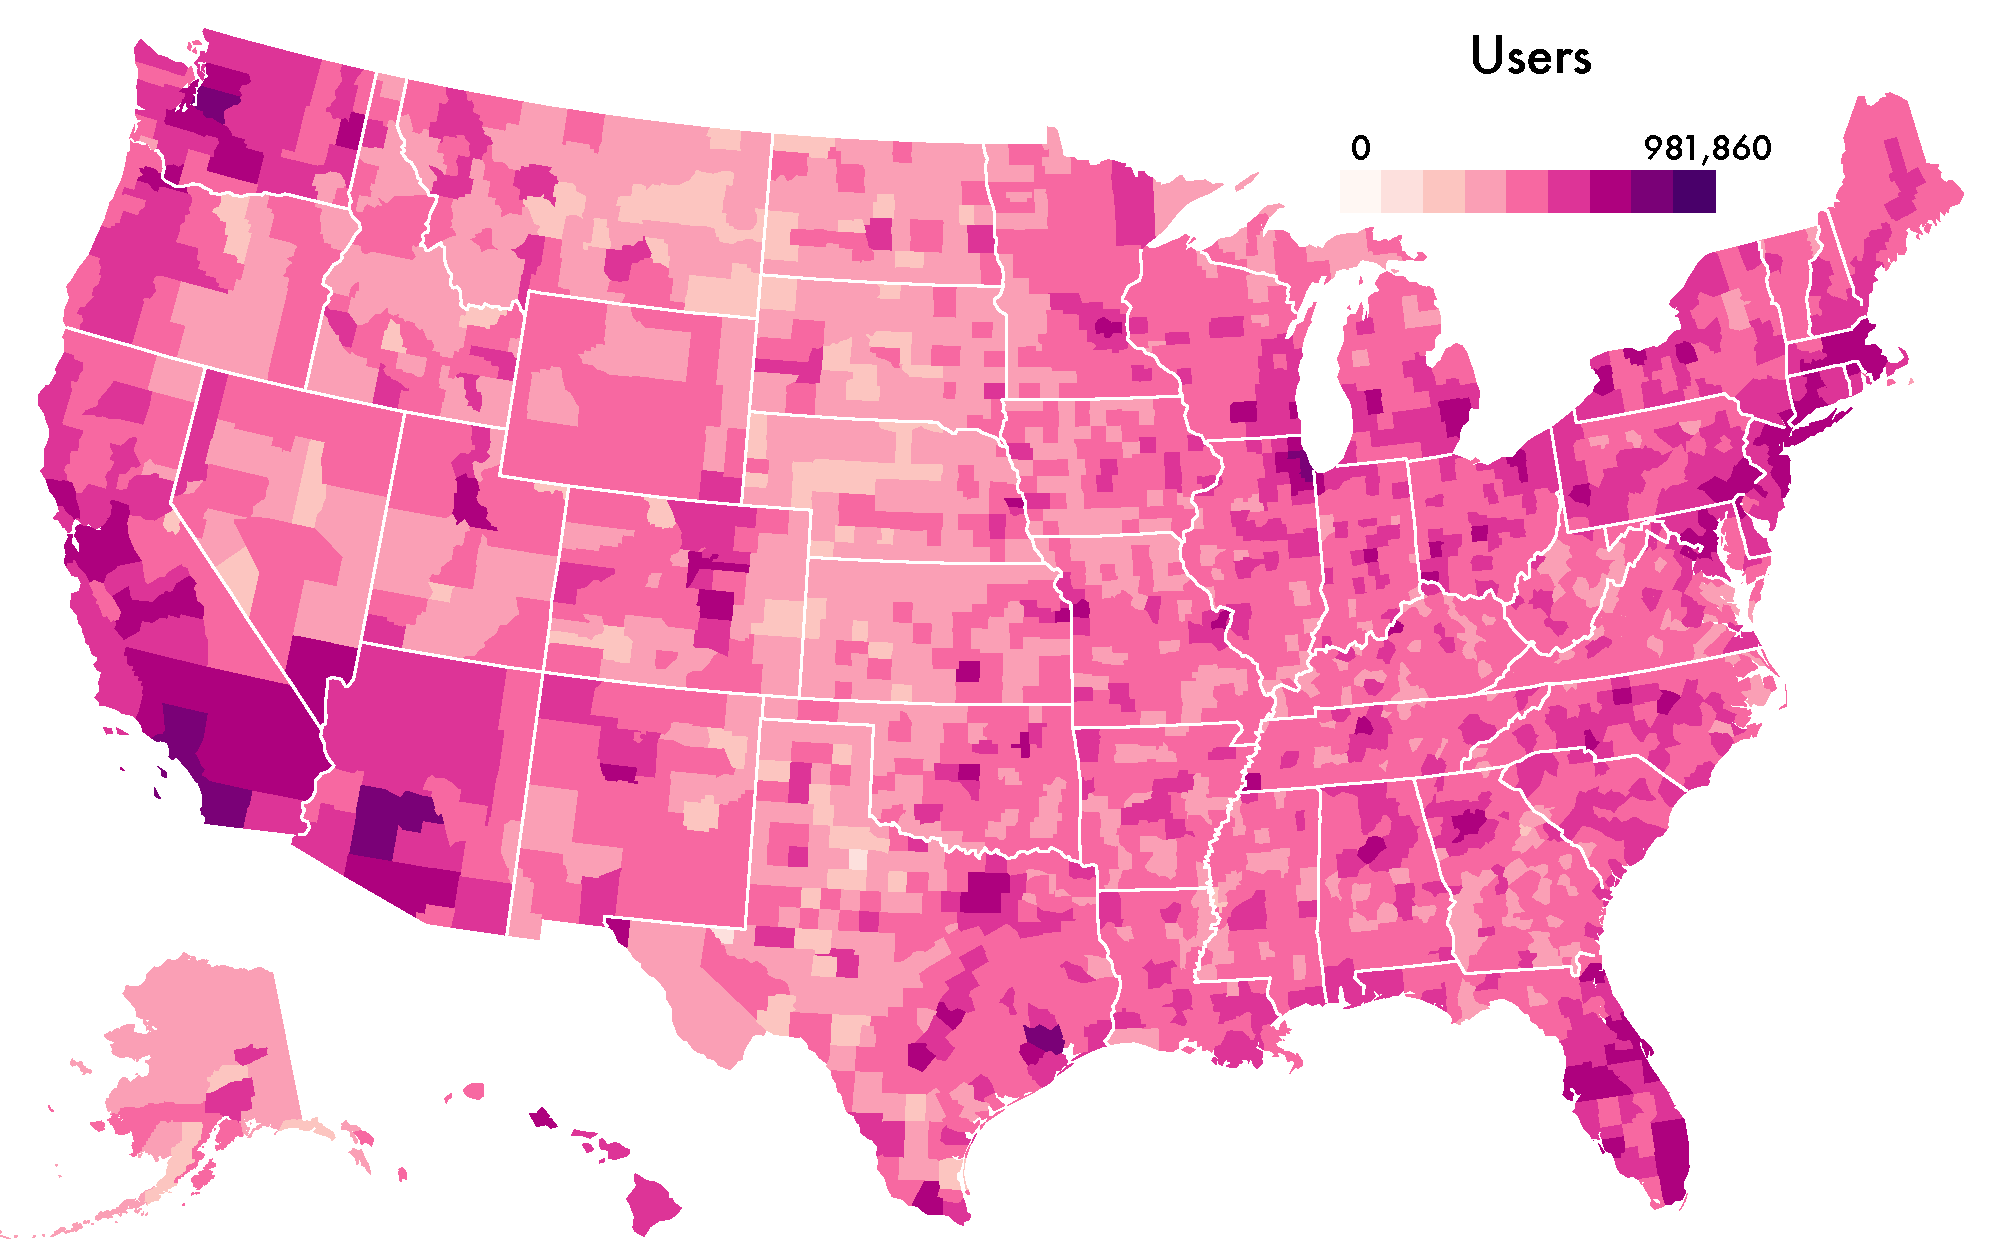
\includegraphics[width=\textwidth]{./figures/population2}
		\caption{Users of Application B}
		\label{fig:pop2}
	\end{subfigure}
	~
	\begin{subfigure}[tb]{0.3\textwidth}
		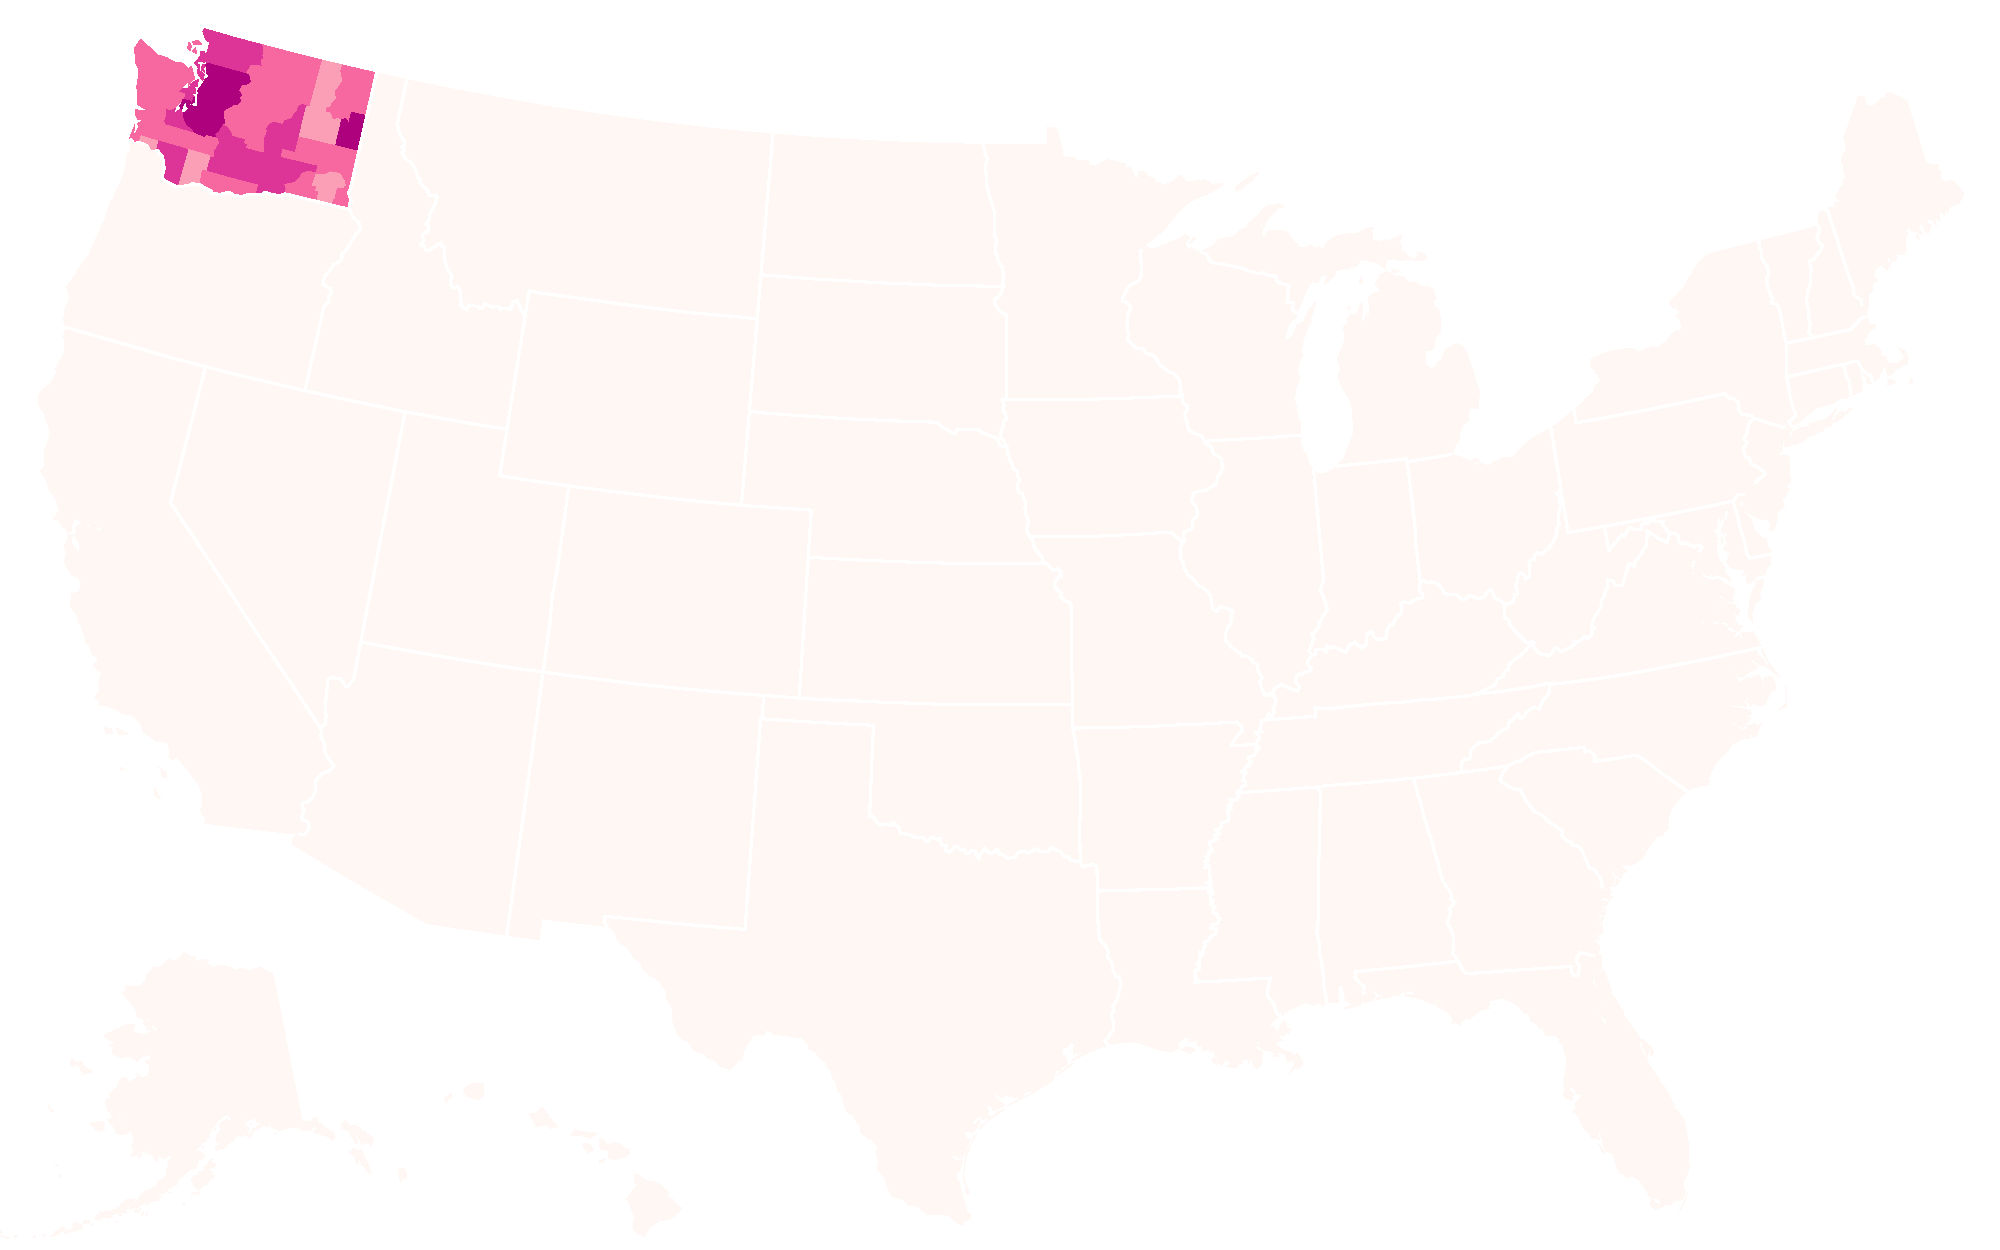
\includegraphics[width=\textwidth]{./figures/population}
		\caption{B-A}
		\label{fig:popdiff}
	\end{subfigure}
	\caption{Choropleth maps illustrating the base rate bias. By encoding only the unweighted density of events, the base rate or population rate of event occurrence is the dominant visual signal, making spatial comparisons difficult. These choropleth maps visualize the location of users of two fictional software applications, A and B. The usage patterns look very similar at a glance, but that is because usage largely follows population (a U.S. citizen is 10\% likely to use either application). An interesting spatial pattern\,---\,B has twice as many users in Washington state as A\,---\,is all but drowned out by the spatially complex, but largely task-irrelevant, signal of U.S. population density.}
	\label{fig:pop}
\end{figure*}
}

\newcommand{\poissonFig}{
\begin{figure*}
	\centering
	\begin{subfigure}[tb]{0.3\textwidth}
		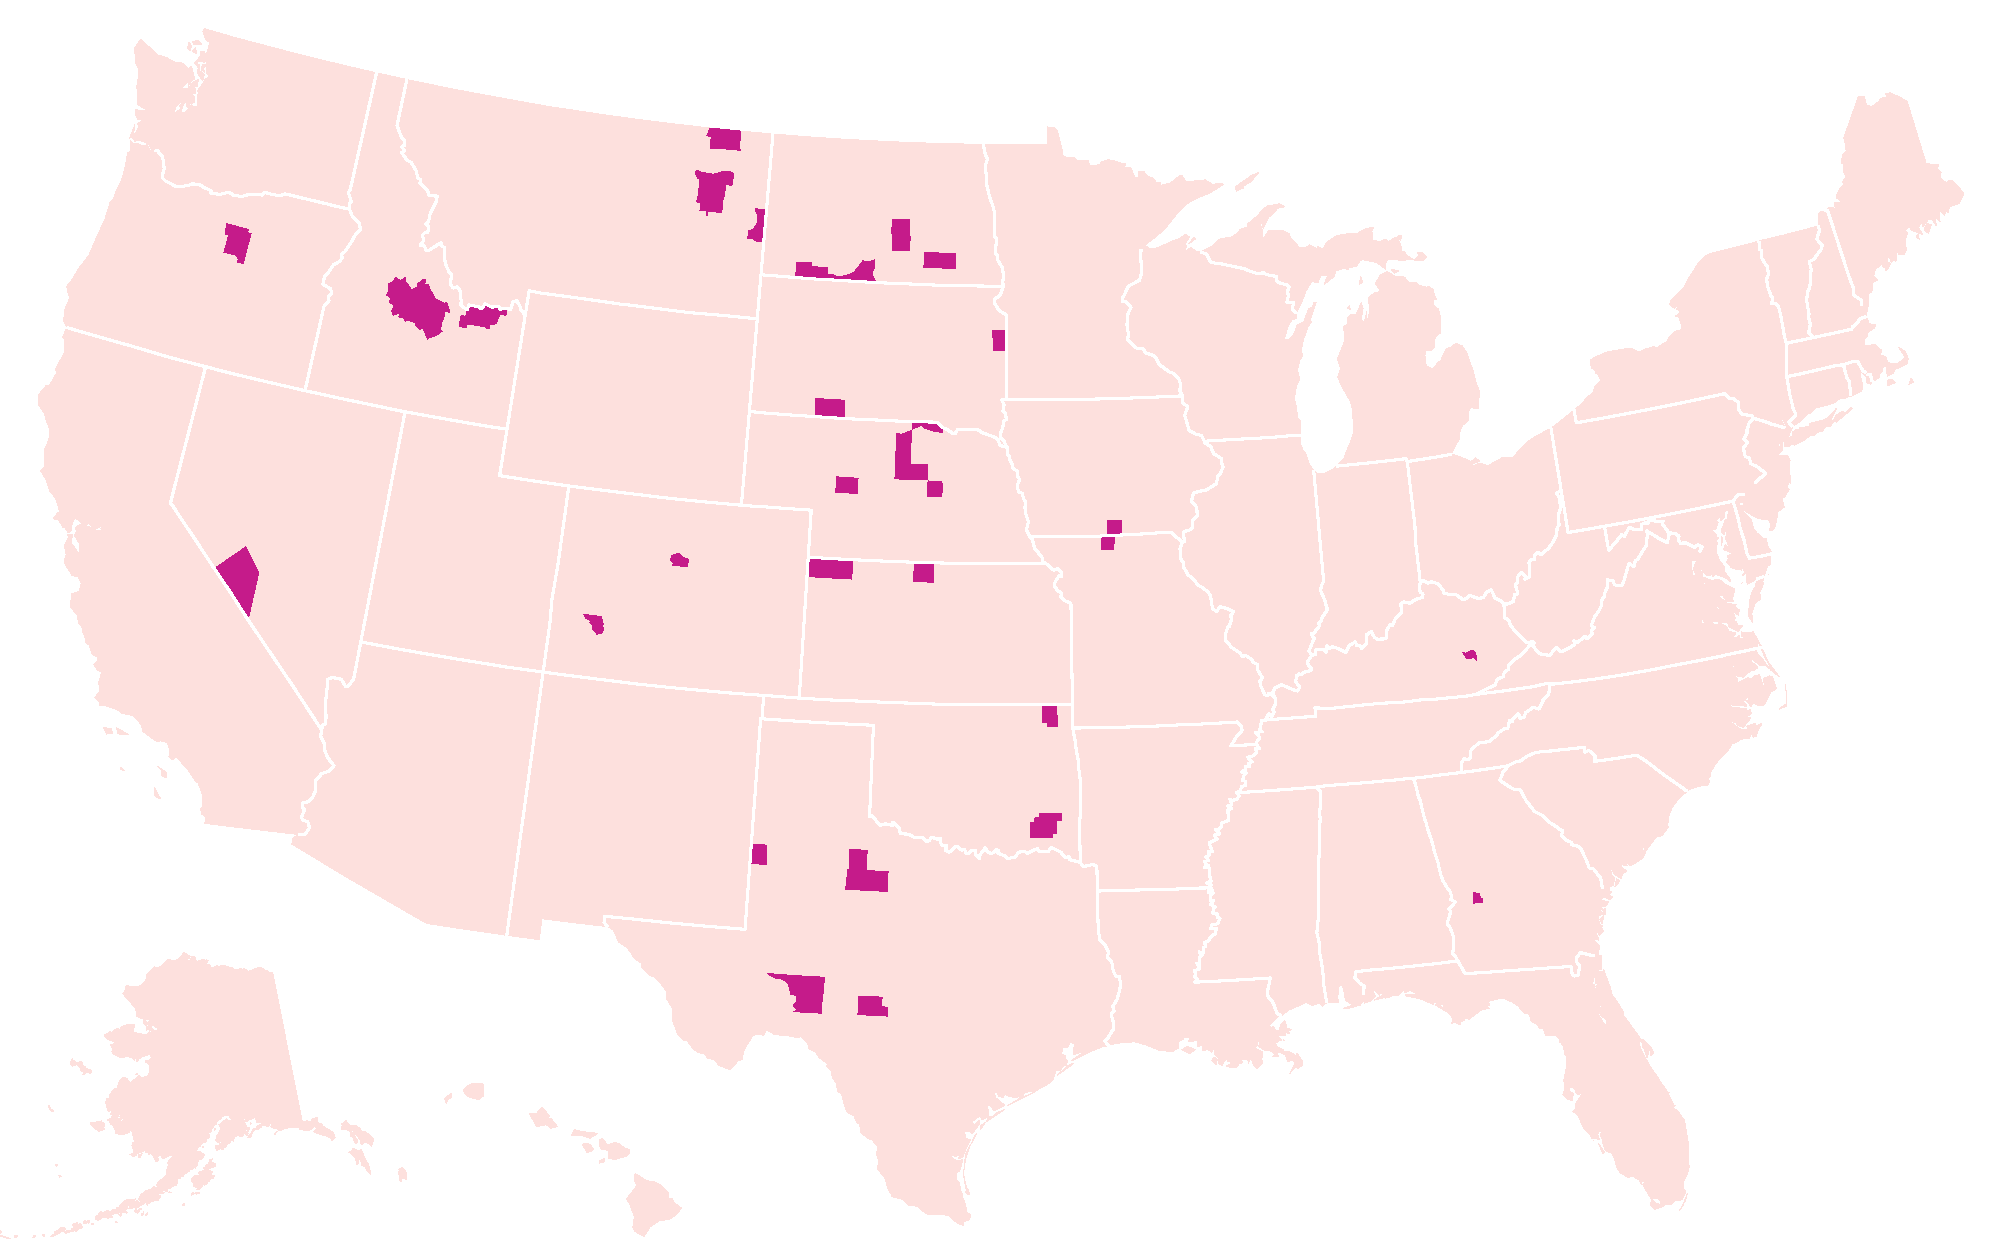
\includegraphics[width=\textwidth]{./figures/poisson-highs}
		\caption{Purple: Bottom 10\% ``Dangerous'' counties.}
		\label{fig:poisson1}
	\end{subfigure}
	~
	\begin{subfigure}[tb]{0.3\textwidth}
		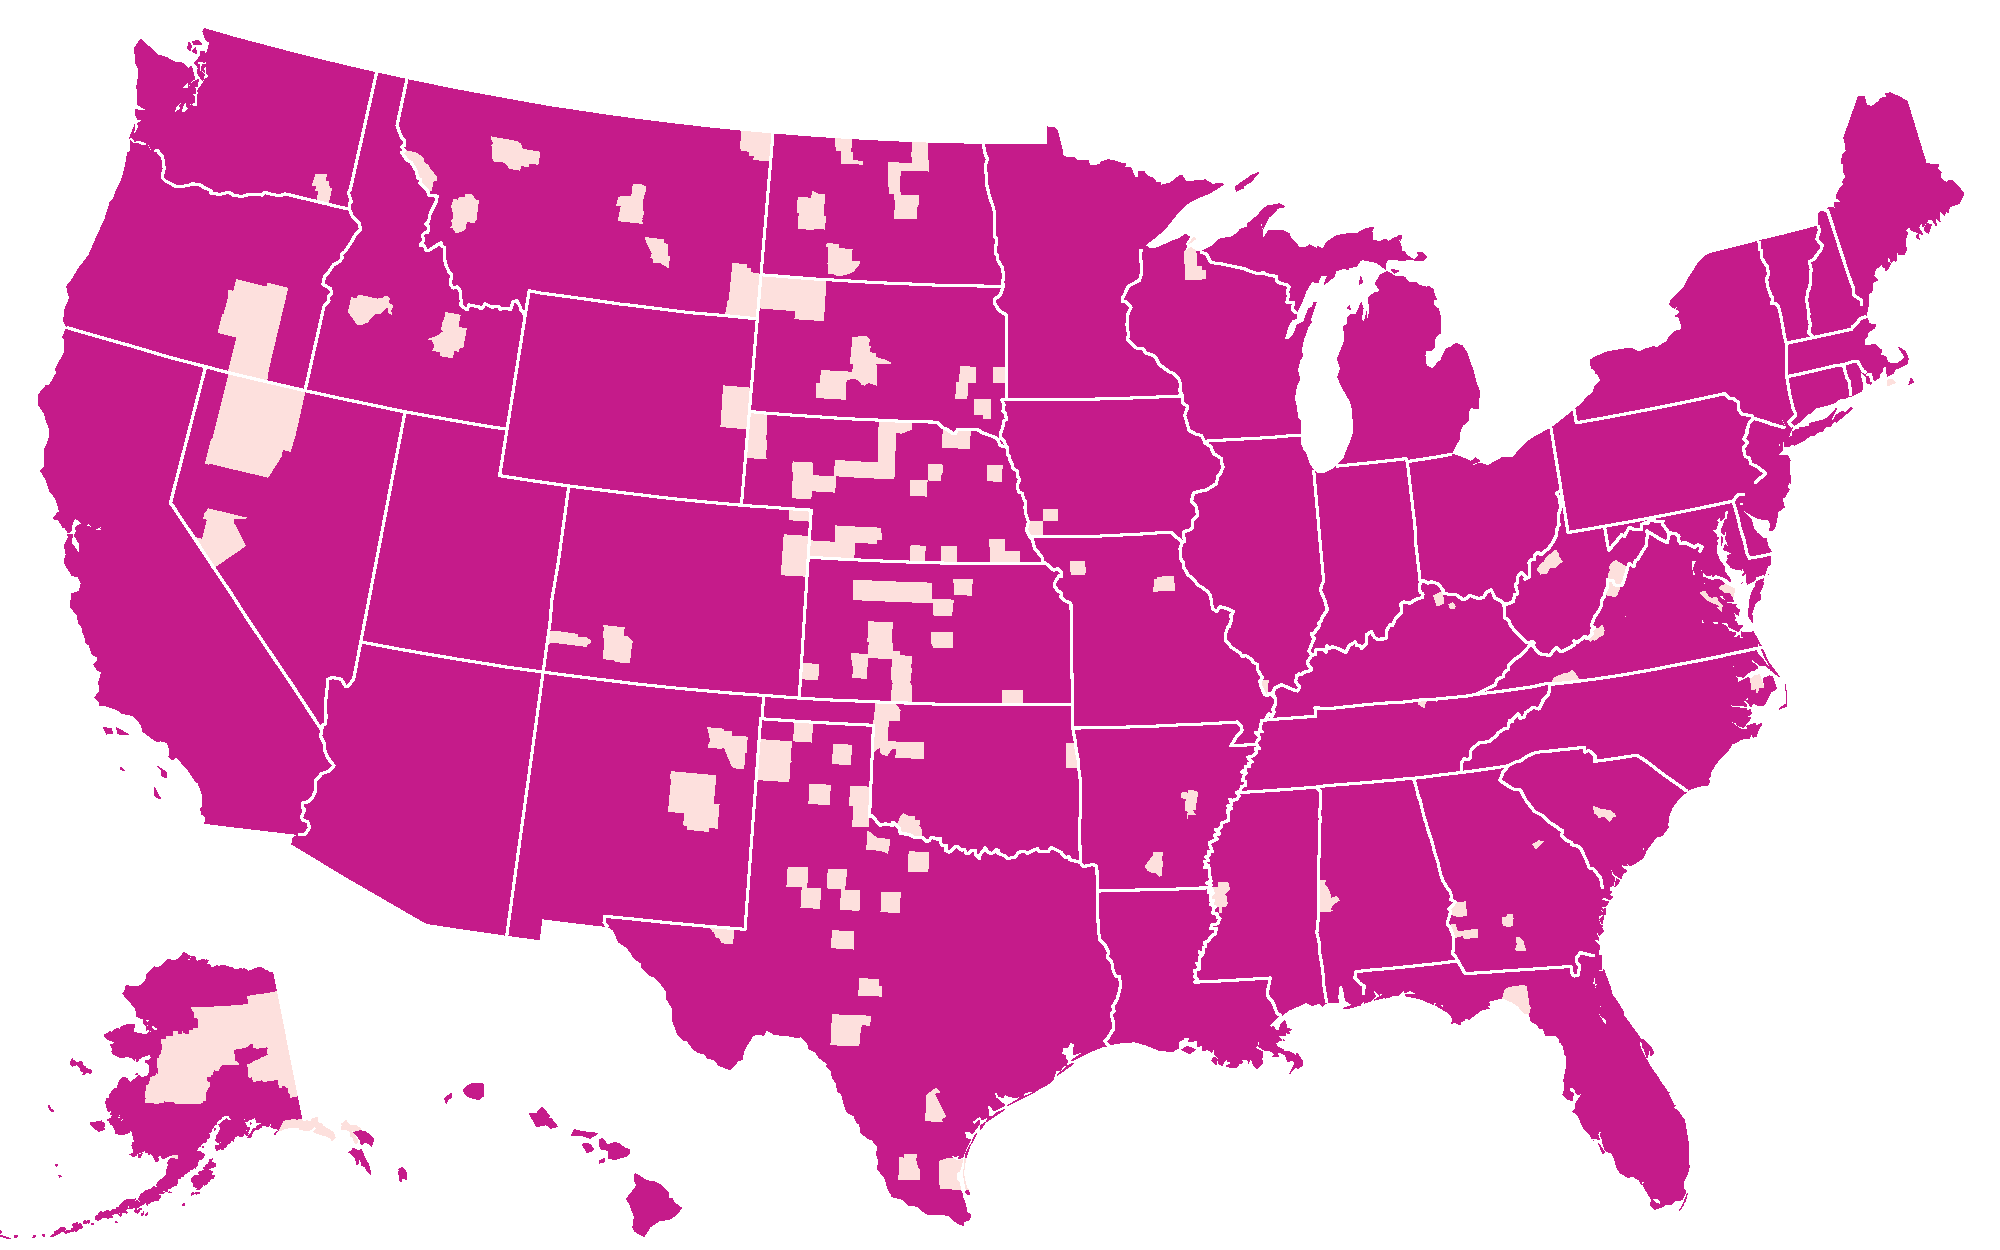
\includegraphics[width=\textwidth]{./figures/poisson-lows}
		\caption{Pink: Top 10\% ``Safe'' counties.}
		\label{fig:poisson2}
	\end{subfigure}
	~
	\begin{subfigure}[tb]{0.3\textwidth}
		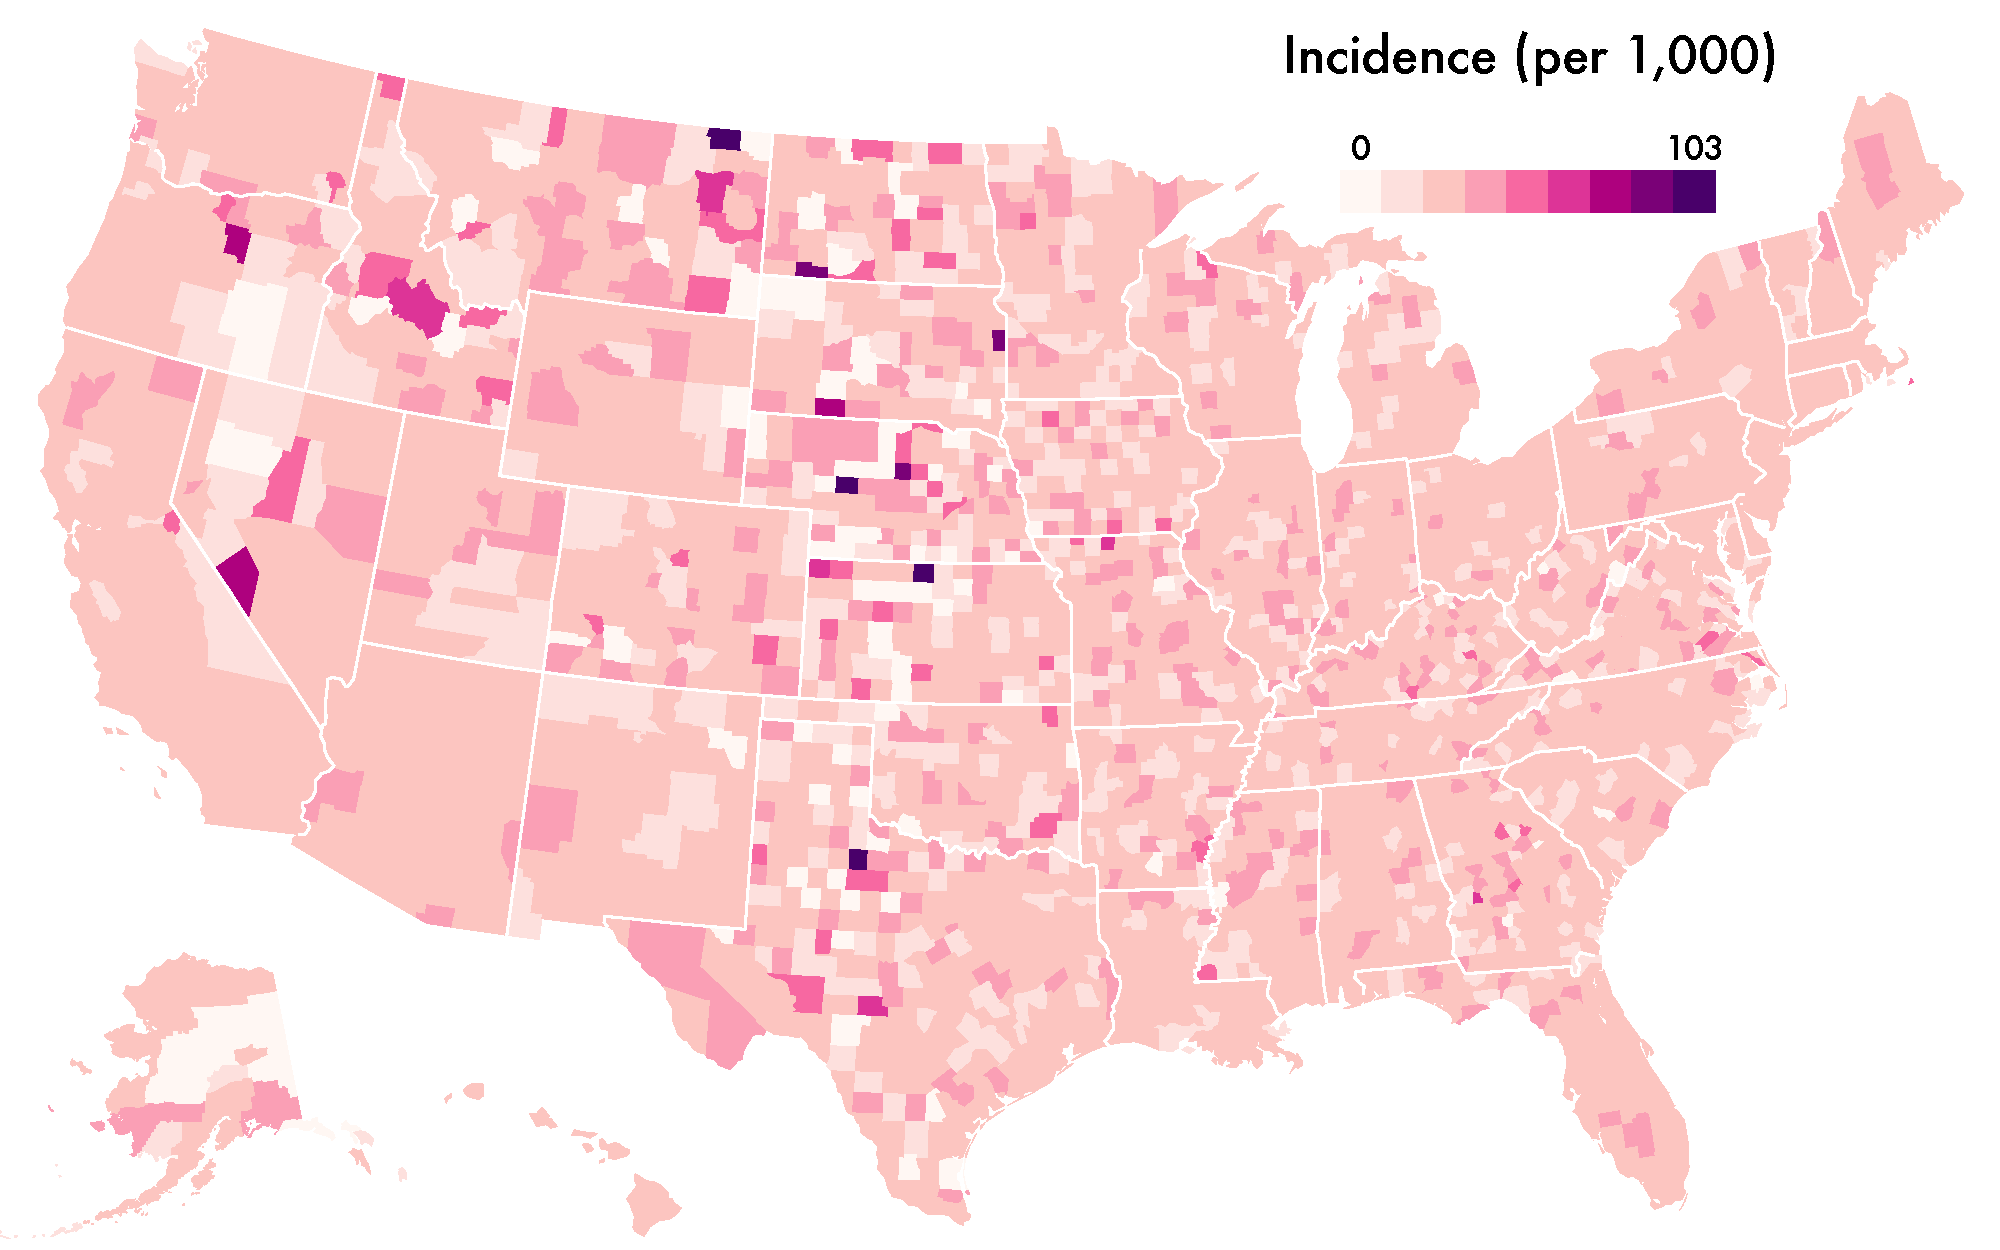
\includegraphics[width=\textwidth]{./figures/poisson}
		\caption{Rates across all counties.}
		\label{fig:poisson3}
	\end{subfigure}
	\caption{Choropleth maps illustrating the sampling error bias. By na\"ively normalizing event density (for instance visualizing per-capita, rather than raw density), latent variables can create erroneous geographic patterns. As an example, low population regions have higher variance than high population regions. These maps encode the per-capita incidence of a fictional disease. (a) The counties with high rates of disease appear localized in the great plains region. However, we also see that (b) the counties with the lowest rates are also mostly located in this region. In fact, the data were generated from a Poisson process with a .1\% chance of infection for each citizen, regardless of location. The apparent geographic patterns are an artifact of (c) the high variance in counties with low population.
	}
	\label{fig:poisson}
\end{figure*}
}

\newcommand{\renormFig}{
\begin{figure*}
	\centering
	\begin{subfigure}[tb]{0.3\textwidth}
		\includegraphics[width=\textwidth]{./figures/renormc}
		\caption{Initial density map.}
		\label{fig:renorm1}
	\end{subfigure}
	~
	\begin{subfigure}[tb]{0.3\textwidth}
		\includegraphics[width=\textwidth]{./figures/renorm-modec}
		\caption{Adding to the mode.}
		\label{fig:renorm2}
	\end{subfigure}
	~
	\begin{subfigure}[tb]{0.3\textwidth}
		\includegraphics[width=\textwidth]{./figures/renorm-outlierc}
		\caption{Adding an outlier.}
		\label{fig:renorm3}
	\end{subfigure}
	\caption{
		Heatmaps illustrating renormalization bias. Incoming data may force renormalization. This readjustment step can be visually disruptive, even though the event itself may not be. (a) A KDE map of events that are normally distributed. (b) Adding events, represented by a Gaussian kernel, to the modal location causes a large visual change to the resulting density map (over 90\% of pixels have a different color value). (c) Adding outlier events to the upper left (arguably a more significant occurrence), only affects the pixels in the region of the outlier (6\% of pixels).
		%If color is continuously mapped to density, this issue is even more pronounced (99\% vs. 6\% of pixel values changed, depending on color gamut).
	}
	\label{fig:renorm}
\end{figure*}
}


\newcommand{\fireFig}{
	\begin{figure}
		\centering
		\includegraphics[width=.9\columnwidth]{figures/fire3-2}
		\caption{
			Signed Surprise Map (left) and KDE density map (right) of 313 fires in northern Los Angeles county, from the spacetime package for R \protect\cite{pebesma2012spacetime}. $\mathcal{M}$ consists of Gaussian, uniform, and sampled subset (first 25 fires) models. Signed surprise is on the interval $[-0.53,0.53]$. The sampled subset model quickly becomes the likeliest model (indicating that fires tend to reoccur in similar spatial regions). The first few fires occurred in the far southwest, with isolated fires in regions in the southeast. Over time, this original spatial mode extends slightly southwards. The Surprise Map highlights this new, dangerous region. The faint blue regions in the southeast show locations where fires occurred in the first 25 events, but not subsequently.
		}
		\label{fig:fire}
	\end{figure}
}


%This example is missing something. I've been playing around with having a bunch of bootstrapped models and then seeing what pops out, but the answer is still "not very much, over the 1000 quakes"

\newcommand{\quakeFig}{
	\begin{figure}
		\centering
		\includegraphics[width=.9\columnwidth]{figures/quake2-2}
		\caption{Signed Surprise Maps (left) and KDE density maps (right) of earthquakes in the South Pacific, near Fiji, from the R datasets package \cite{rdatasets}. $\mathcal{M}$ consists of Gaussian, uniform, and sampled subset (in this case a bootstrapped sample of 50 events) models. Signed surprise is from $[-0.53,0.53]$. The bootstrapped model eventually becomes the most likely, reflecting long-term homogeneity in quake location. However, small differences in density (such as the red region south of Fiji with higher than expected quake density), are highlighted in the Surprise maps, allowing more focused comparison across timepoints.
		}
		\label{fig:quake}
	\end{figure}
}

\newcommand{\quakeFigvTwo}{
	\begin{figure}[htb]
		\centering
		\begin{subfigure}[t]{.35\textwidth}
			\includegraphics[width=\textwidth]{figures/quake1-2}
			\caption{Signed Surprise and KDE Density after 100 events. }
			\label{fig:quake2-1}
		\end{subfigure}

		\begin{subfigure}[t]{.35\textwidth}
			\includegraphics[width=\textwidth]{figures/quake2-2}
			\caption{Signed Surprise and KDE Density after 1,000 events.}
			\label{fig:quake2-2}
		\end{subfigure}

		\caption{Signed Surprise Maps (1st and 3rd from left) and KDE density maps (2nd and 4th from left) of earthquakes in the South Pacific, near Fiji, from the R datasets package \cite{rdatasets}, after 100 (Fig. \ref{fig:quake2-1}) and 1,000 (Fig. \ref{fig:quake2-2}) events. $\mathcal{M}$ consists of Gaussian, uniform, and sampled subset (in this case a bootstrapped sample of 50 events) models. Signed surprise is from $[-0.53,0.53]$. The bootstrapped model eventually becomes the most likely, reflecting long-term homogeneity in quake location. This homogeneity makes it difficult to compare densities using a traditional KDE map. Bootstrapped models afford comparison to a sampled representation of the whole, highlighting differences such as the underrepresentation of northern quakes after 100 events.
		}
		\label{fig:quake2}
	\end{figure}
}


\newcommand{\unemploymentFig}{
	\begin{figure}
		\centering
		\begin{subfigure}[t]{.9\columnwidth}
			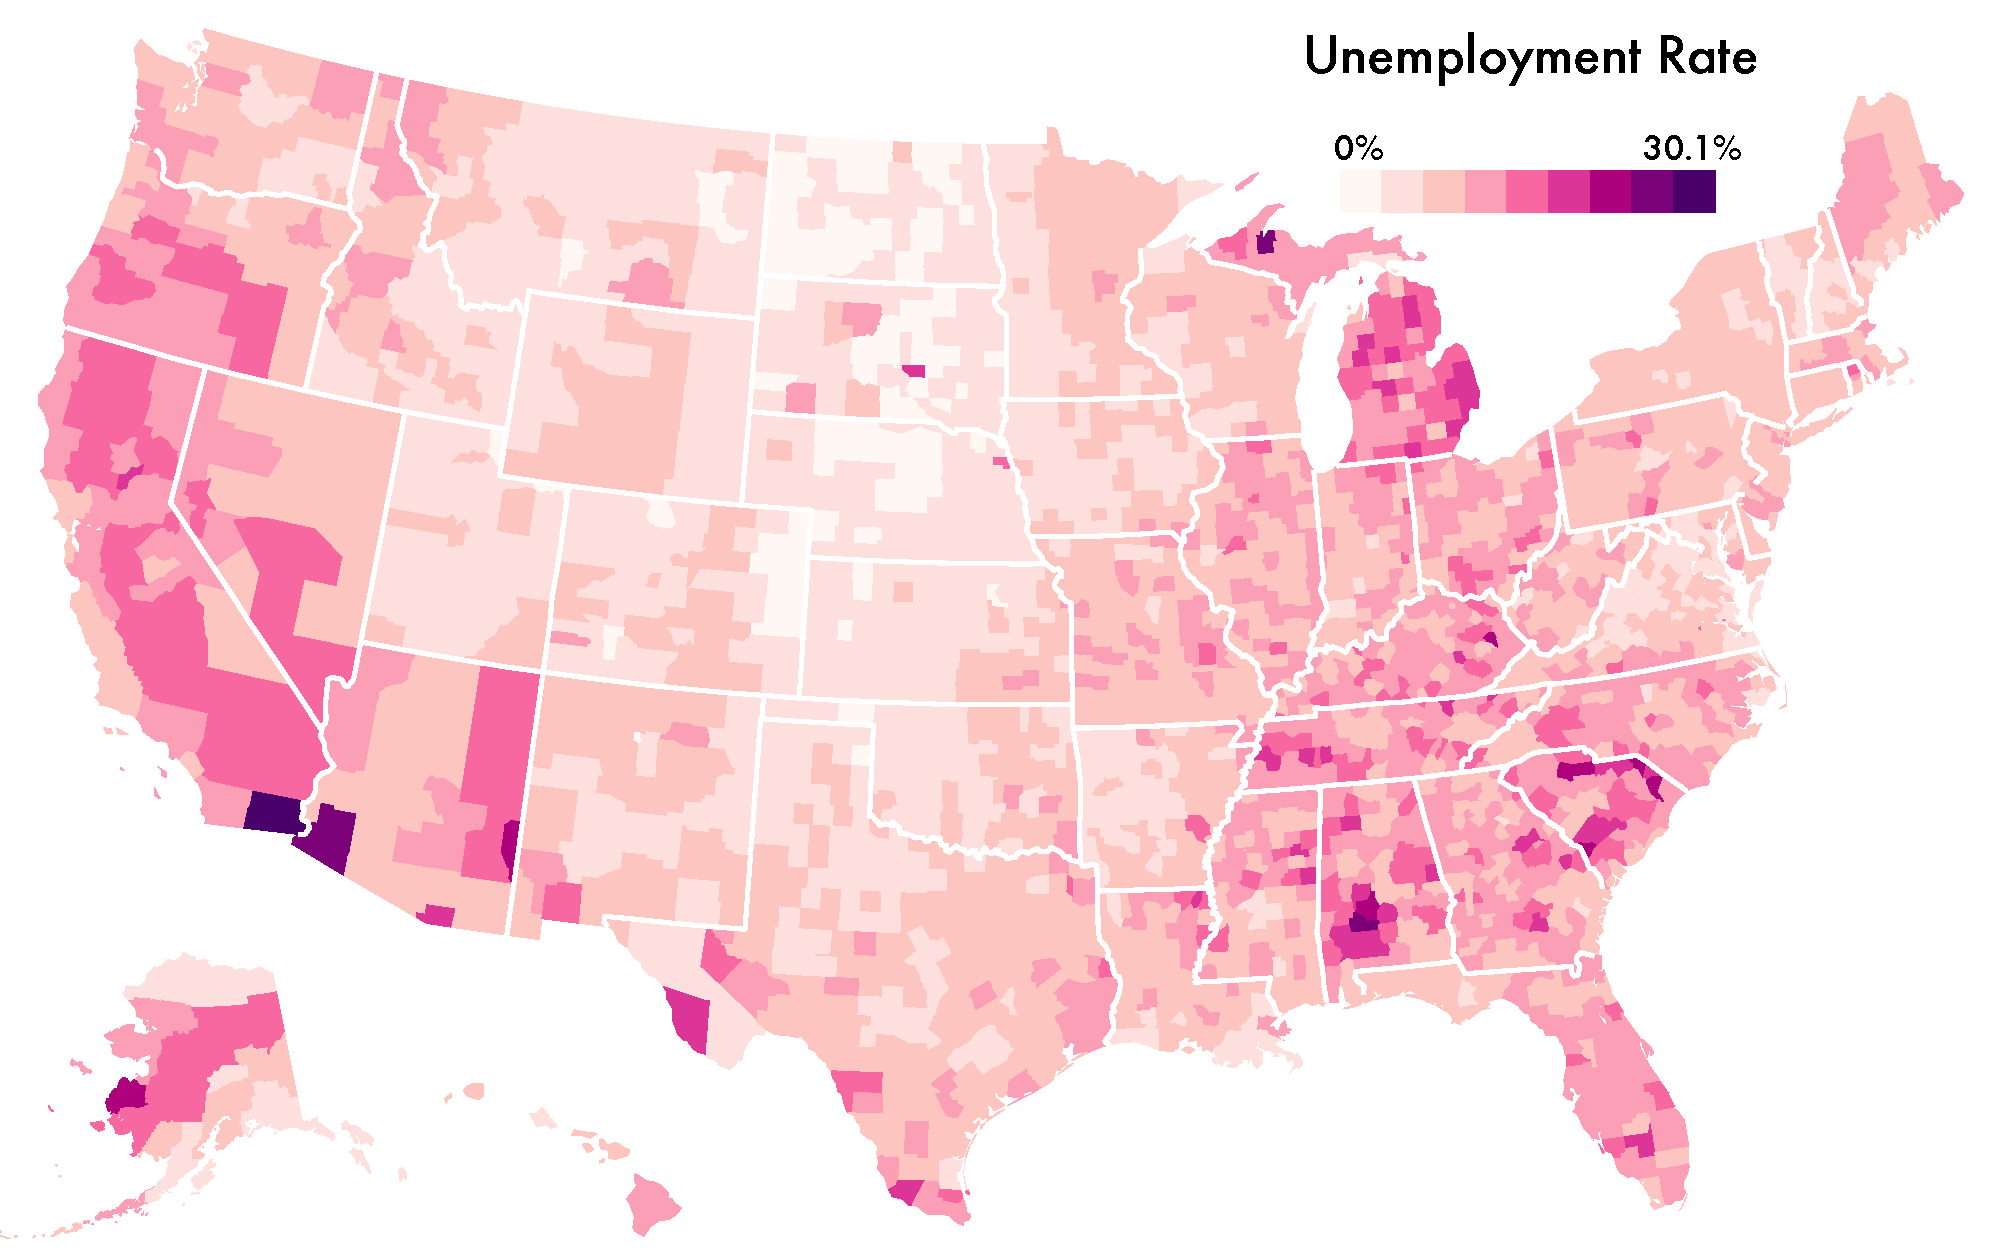
\includegraphics[width=\textwidth]{figures/unemployment2}
			\caption{Per capita event rate map. }
			\label{fig:unemployment1}
		\end{subfigure}

		\begin{subfigure}[t]{.9\columnwidth}
			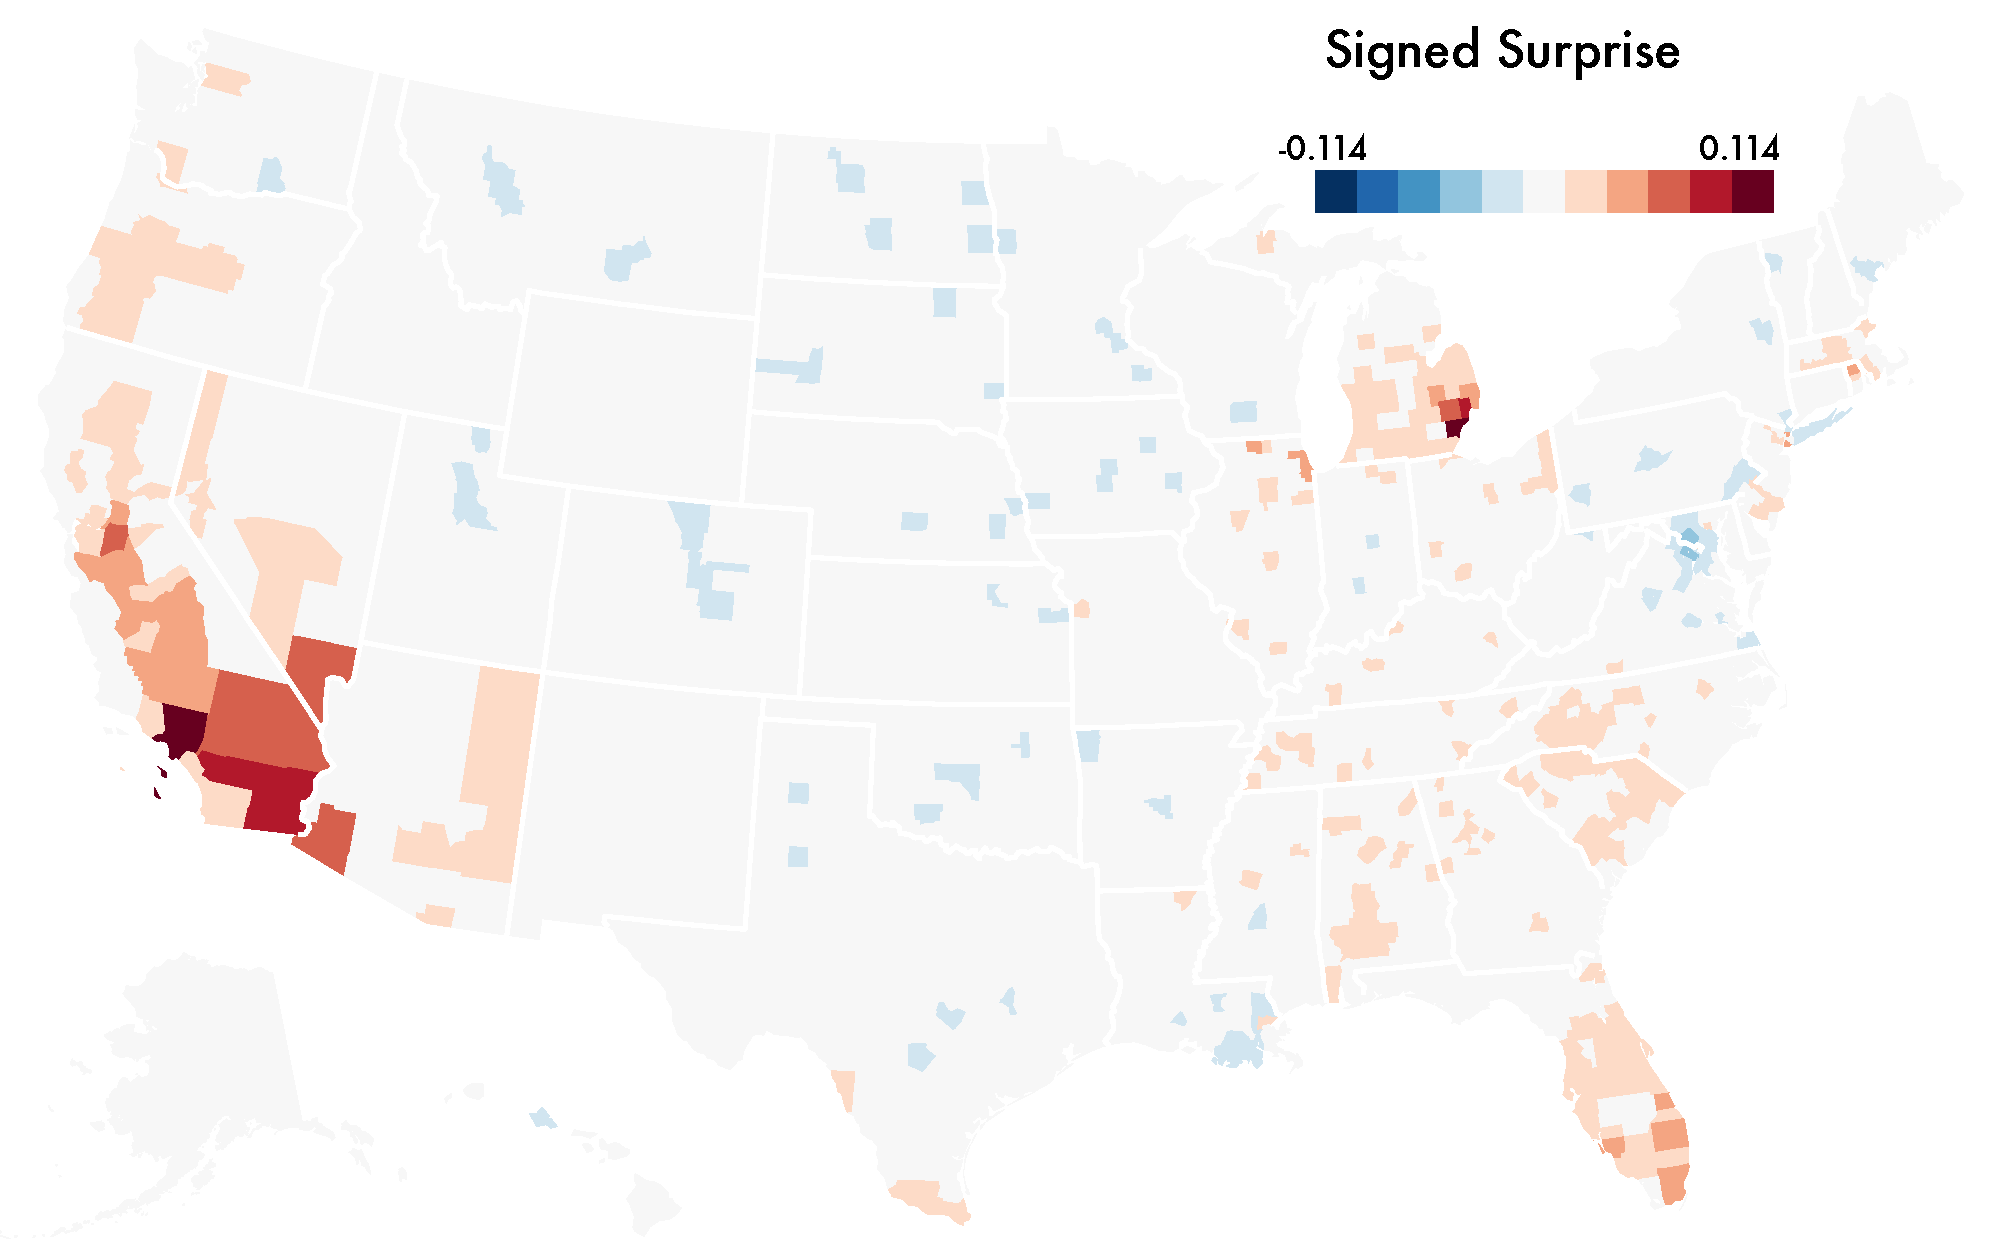
\includegraphics[width=\textwidth]{figures/unemployment-surprise}
			\caption{Signed Surprise Map. }
			\label{fig:unemployment2}
		\end{subfigure}
		\caption{Comparing a traditional map of the 2008 per-capita unemployment rate (Fig. \protect\ref{fig:unemployment1}) with a Surprise Map (Fig. \protect\ref{fig:unemployment2}). $\mathcal{M}$ is a population model and a de Moivre funnel (see Fig. \protect\ref{fig:funnel}) for details. The traditional map seems to show that the great plains region has particularly low unemployment, but the low populations in these regions make those data unreliable. Down-weighting sparse counties with high variance, the Surprise Map shows robustly high unemployment in the Los Angeles and the Detroit metro areas. The Washington D.C. metro area has surprisingly low unemployment, perhaps due to the many jobs provided by the Federal government and related agencies.
		}
		\label{fig:unemployment}
	\end{figure}
}

\newcommand{\coasstFig}{
	\begin{figure*}
		\centering
		\begin{subfigure}[t]{.3\textwidth}
			\includegraphics[width=\textwidth]{figures/coasst-observed}
			\caption{Bird death event rate map. }
			\label{fig:coasst1}
		\end{subfigure}
		~
		\begin{subfigure}[t]{.3\textwidth}
		\includegraphics[width=\textwidth]{figures/coasst-normalized}
		\caption{Per species normalized bird death map. }
		\label{fig:coasstn}
		\end{subfigure}
		~
		\begin{subfigure}[t]{.3\textwidth}
			\includegraphics[width=\textwidth]{figures/coasst-surprise}
			\caption{Signed Surprise Map. }
			\label{fig:coasst2}
		\end{subfigure}
		\caption{Comparing event density (Fig. \protect\ref{fig:coasst1}) and event rate (Fig. \protect\ref{fig:coasstn}) maps of 2014 per-species surveyed bird deaths  with a Surprise Map (Fig. \protect\ref{fig:coasst2}). Data comes from the COASST beached bird dataset \protect\cite{coasst}. $\mathcal{M}$ is a population model based on data from 1999-2015, and a seasonal model based on per-month variation. Signed surprise is from $[-0.9,0.9]$. Common species families like gulls and alcids (puffins) dominate the density map, making it difficult to reason about non-modal species. The normalized rate map allows analysts to better distinguish intra-species patterns, but hides deviations from seasonal patterns, such as the uncommonly low death rate of Small Alcids in January (0.15\% of all 2014 Small Alcid deaths): normally, 40.56\% of Small Alcid deaths occur in January.
		}
		\label{fig:coasst}
	\end{figure*}
}